
\documentclass[12pt]{article}

% Layout.
\usepackage[top=1in, bottom=0.75in, left=1in, right=1in, headheight=1in, headsep=6pt]{geometry}

% Fonts.
\usepackage{mathptmx}
\usepackage[scaled=0.86]{helvet}
\renewcommand{\emph}[1]{\textsf{\textbf{#1}}}

% TiKZ.
\usepackage{tikz, pgfplots}
\usetikzlibrary{calc}
\pgfplotsset{compat = newest}
 
\pgfplotsset{my style/.append style={axis x line=middle, axis y line=
middle, xlabel={$x$}, ylabel={$y$}, axis equal }}

% Misc packages.
\usepackage{amsmath,amssymb,latexsym}
\usepackage{graphicx}
\usepackage{array}
\usepackage{xcolor}
\usepackage{multicol}

% Commands to set various header/footer components.
\makeatletter
\def\doctitle#1{\gdef\@doctitle{#1}}
\doctitle{Use {\tt\textbackslash doctitle\{MY LABEL\}}.}
\def\docdate#1{\gdef\@docdate{#1}}
\docdate{Use {\tt\textbackslash docdate\{MY DATE\}}.}
\def\doccourse#1{\gdef\@doccourse{#1}}
\let\@doccourse\@empty
\def\docscoring#1{\gdef\@docscoring{#1}}
\let\@docscoring\@empty
\def\docversion#1{\gdef\@docversion{#1}}
\let\@docversion\@empty
\makeatother

% Headers and footers layout.
\makeatletter
\usepackage{fancyhdr}
\pagestyle{fancy}
\fancyhf{} % Clears all headers/footers.
\lhead{\baselineskip 30pt
%\emph{\@doctitle\hfill\@docdate}
\emph{\@docdate\hfill\@doctitle}
\ifnum \value{page} > 1\relax\else\\
\emph{Name: \rule{3.5in}{1pt}\hfill \@docscoring}\fi}
\rfoot{\emph{\@docversion}}
\lfoot{\emph{\@doccourse}}
\cfoot{\emph{\thepage}}
\renewcommand{\headrulewidth}{0pt}%
\makeatother

% Paragraph spacing
\parindent 0pt
\parskip 6pt plus 1pt

% A problem is a section-like command. Use \problem{5} to
% start a problem worth 5 points.
\newcounter{probcount}
\newcounter{subprobcount}
\setcounter{probcount}{0}
\newcommand{\problem}[1]{%
\par
\addvspace{4pt}%
\setcounter{subprobcount}{0}%
\stepcounter{probcount}%
\makebox[0pt][r]{\emph{\arabic{probcount}.}\hskip1ex}\emph{[#1 points]}\hskip1ex}
\newcommand{\thesubproblem}{\emph{\alph{subprobcount}.}}

% Subproblems are an enumerate-like environment with a consistent
% numbering scheme. 
% Use \begin{subproblems}\item...\item...\end{subproblems}
\newenvironment{subproblems}{%
\begin{enumerate}%
\setcounter{enumi}{\value{subprobcount}}%
\renewcommand{\theenumi}{\emph{\alph{enumi}}}}%
{\setcounter{subprobcount}{\value{enumi}}\end{enumerate}}

% Blanks for answers in normal and math mode.
\newcommand{\blank}[1]{\rule{#1}{0.75pt}}
\newcommand{\mblank}[1]{\underline{\hspace{#1}}}
\def\emptybox(#1,#2){\framebox{\parbox[c][#2]{#1}{\rule{0pt}{0pt}}}}

% Misc.
\renewcommand{\d}{\displaystyle}
\newcommand{\ds}{\displaystyle}
\def\bc{\begin{center}}
\def\ec{\end{center}}
\def\be{\begin{enumerate}}
\def\ee{\end{enumerate}}


\doctitle{Math 251: Quiz 2}
\docdate{September 5, 2024}
\doccourse{UAF Calculus I}
\docversion{v-1}
\docscoring{\blank{0.8in} / 25}
\begin{document}
%\textbf{Please circle your instructor's name:} \hfill Leah Berman  \hfill   Jill Faudree\\

There are 25 points possible on this quiz. No aids (book, calculator, etc.)
are permitted.  {\bf Show all work for full credit.}

\problem{11} Let $P(2,2)$ be a point on the graph of $f(x)=\displaystyle{\frac{6-x}{x}}.$
\begin{subproblems}
\item Find the slope of the secant line passing through $P$ and the point $Q(1,f(1)).$ 
\vfill

\item Find the slope of the secant line passing through $P$ and the point $Q(3,f(3)).$

\vfill

\item The table below lists the slope of the secant line passing through the point $P$ and the point $Q(x, f(x))$ for several values of $x.$ \\

\begin{tabular}{l || c|c|c|c|c|c}
x&1.9&1.99&1.999&2.001&2.01&2.1\\
\hline
f(x)&2.157895&2.015075&2.001501&1.998501&1.985075&1.857143 \\
\hline
$m_{sec}$&-1.57895 &-1.50754&-1.50075&-1.49925&-1.49254&-1.42857\\
\end{tabular}

\vskip 0.5cm
Use the information in the table to estimate the slope of the tangent line to $f(x)$ at the point $P(2,2).$
\vfill

\item Use the slope from part (c) above to write an equation of the tangent line at point $P(2,2).$

\vfill

\item Below is a sketch of the graph of $f(x)=\frac{6-x}{x}.$ Sketch the tangent line to the graph at the point $P(2,2).$

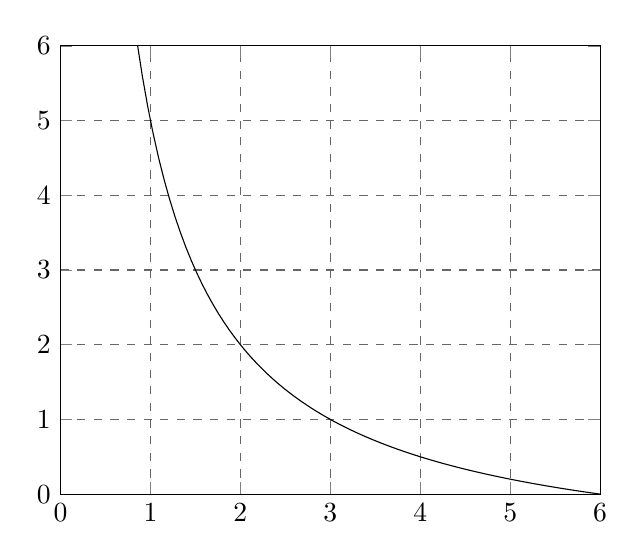
\begin{tikzpicture}
 \begin{axis}[
    xmin = 0, xmax = 6,
    ymin = 0, ymax = 6, xtick={0,1,...,6}, ytick={0,1,...,6},
    grid=both, grid style={ thin, black!60, dashed}]
    \addplot[samples=100,
        domain = 0:6,
    ] {(6-x)/(x)};
    %\addplot[thick,->] coordinates {(-1,0) (6,0)};
\end{axis}
\end{tikzpicture}

\end{subproblems}



\newpage

\problem{14}
A spring is stretched out and released. Its length in inches at time $t$ seconds is given by the function: $$L(t)=4\cos(\pi t) + 6$$.
\begin{subproblems}
\item Sketch a graph of $L(t)$ below. (Hint: Find $L(0), L(1), L(2), L(3),$ and $L(4)$.)

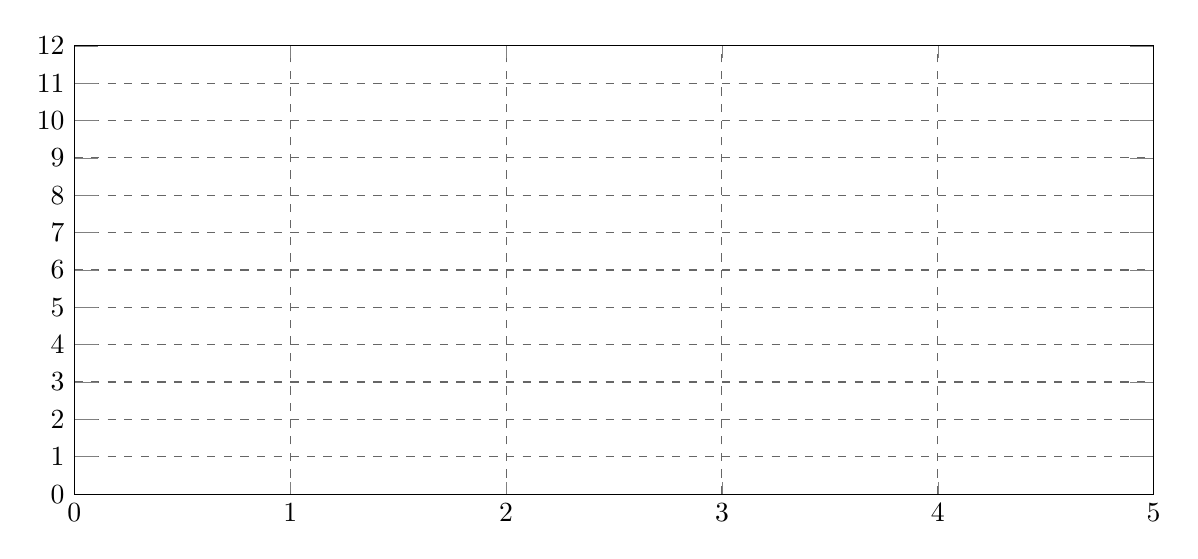
\begin{tikzpicture}
 \begin{axis}[
    xmin = 0, xmax = 5, xscale=2,
    ymin = 0, ymax = 12, xtick={0,1,...,5}, ytick={0,1,...,12},
    grid=both, grid style={ thin, black!60, dashed}];
    %\addplot[thick,->] coordinates {(-1,0) (6,0)};
\end{axis}
\end{tikzpicture}

\item Calculate the length of the spring at $t=\displaystyle \frac{1}{3}$ seconds and $t=\displaystyle \frac{2}{3}$ seconds. Include units in your final answer.\\

\vspace{.3in}

$L\left(\frac{1}{3}\right)=$

\vspace{.2in}

$L\left(\frac{2}{3}\right)=$

\vspace{.2in}

\item Calculate the \textbf{average rate of change} of the length of the spring from $t=\displaystyle \frac{1}{3}$ seconds to $t=\displaystyle \frac{2}{3}$ seconds. Show your work and include units in your final answer.

\vfill

\item Based on your graph in part (a) from above, estimate the \textbf{instantanous rate of change} of the length of the spring at $t=2$ seconds. Unclude units in your final answer.

\vfill


\end{subproblems}


\end{document}